\documentclass[11pt,a4paper]{article}
\usepackage[a4paper, total={7in, 10.25in}]{geometry}


\usepackage{color}
\usepackage{graphicx}
\usepackage{wrapfig}
\usepackage{fancyhdr}
\usepackage{tocloft}
\usepackage{multicol}
\usepackage{hyperref}
\usepackage{tabularx}
\usepackage{array}
\usepackage[export]{adjustbox}
\usepackage{listings}
\usepackage{xcolor}
    \definecolor{codegreen}{rgb}{0,0.6,0}
    \definecolor{codegray}{rgb}{0.5,0.5,0.5}
    \definecolor{codepurple}{rgb}{0.58,0,0.82}
    \definecolor{backcolour}{rgb}{1,1,1}

    \lstdefinestyle{mystyle}{
        backgroundcolor=\color{backcolour},   
        commentstyle=\color{codegreen},
        keywordstyle=\color{magenta},
        numberstyle=\tiny\color{codegray},
        stringstyle=\color{codepurple},
        basicstyle=\ttfamily\footnotesize,
        breakatwhitespace=false,         
        breaklines=true,                 
        captionpos=b,                    
        keepspaces=false,                 
        numbers=left,                    
        numbersep=5pt,                  
        showspaces=false,                
        showstringspaces=false,
        showtabs=false,                  
        tabsize=2
    }



\renewcommand{\cftsecleader}{\cftdotfill{\cftdotsep}}
\graphicspath{ {./images/} }
\hypersetup{
    colorlinks=true,
    linkcolor=blue,
    citecolor=black,
    filecolor=magenta,      
    urlcolor=cyan,
    pdftitle={Overleaf Example},
    pdfpagemode=FullScreen,
    }
\pagestyle{fancy}
\setlength{\headheight}{18pt}
\fancyhead[L]{\textit{EN3551 Digital Signal Processing : Assignment 01}}
\fancyfoot[L]{\textit{Department of Electronic and Telecommunication \\University of Moratuwa}}

\title{DEPARTMENT OF ELECTRONIC AND TELECOMMUNICATION
UNIVERSITY OF MORATUWA

\vspace{10pt}

{\large{\textsc{EN3551 Digital Signal Processing}}}

{\textsf{This is offered as a "EN3551 Digital Signal Processing" module's partial completion.}}

\vspace{30pt}

\includegraphics[scale=1.20]{images/University_of_Moratuwa_logo.png}

{\textsf{\textbf{Assignment 01 : Detecting Harmonics in Noisy Data and Signal Interpolation using DFT}}}}


\author{200686J : Vishagar A.}

\date{$9^{th}$ of september, 2023}

\begin{document}

\maketitle

\newpage

\begin{abstract}
    \textit{This report deals with the explanation of the solutions for the given questions in the assignment 01 of the EN3150 module. The solutions are explained in a way that it is easy to understand and follow. The solutions are explained with the help of the code snippets and the results. We are mainly focussed on some real world problems like "Detecting harmonics from a noisy data" and "Interpolation using DFT". \textbf{And I have used \underline{python} as the programming language to find the solutions for the given problems.}}    
\end{abstract}    

\vspace{50pt}
\tableofcontents


\newpage

\twocolumn

\section{Detecting Harmonics in Noisy Data}

In this section we were given with a signal with four harmonics added with a heavy noise to find the harmonic frequency of the signal using Discrete Fourier Transform. 
Therefore to find these harmonics we were asked to use \textbf{DFT Averaging} technique.\\
\\


{\begin{figure}[h]
    \centering
    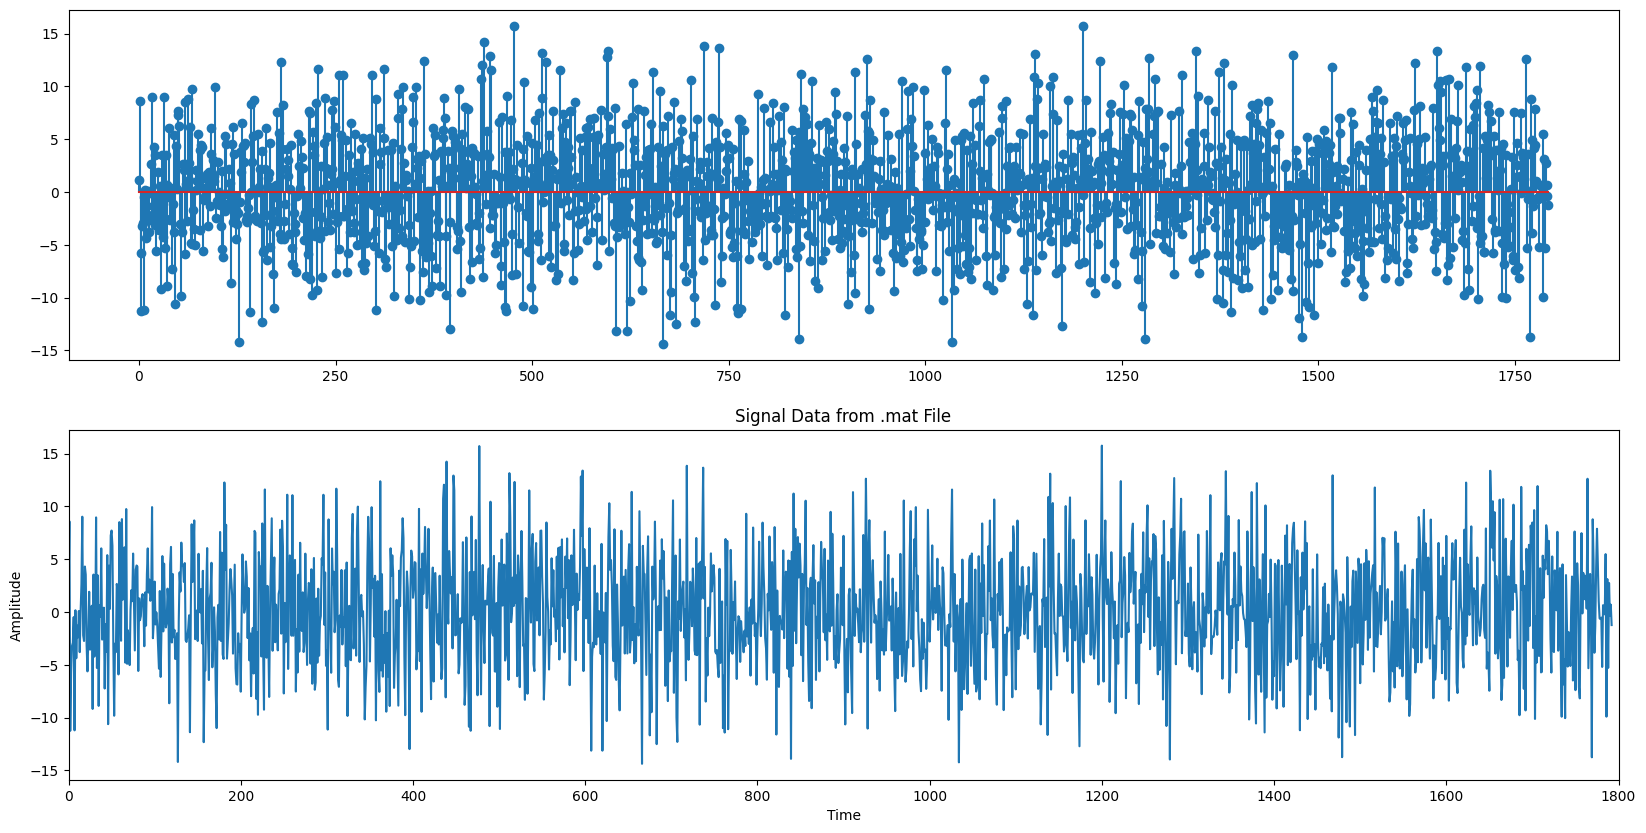
\includegraphics[width=1.0\linewidth]{images/1.png}
    \caption{Provided sample file}
\end{figure}}

{\begin{figure}[h]
    \centering
    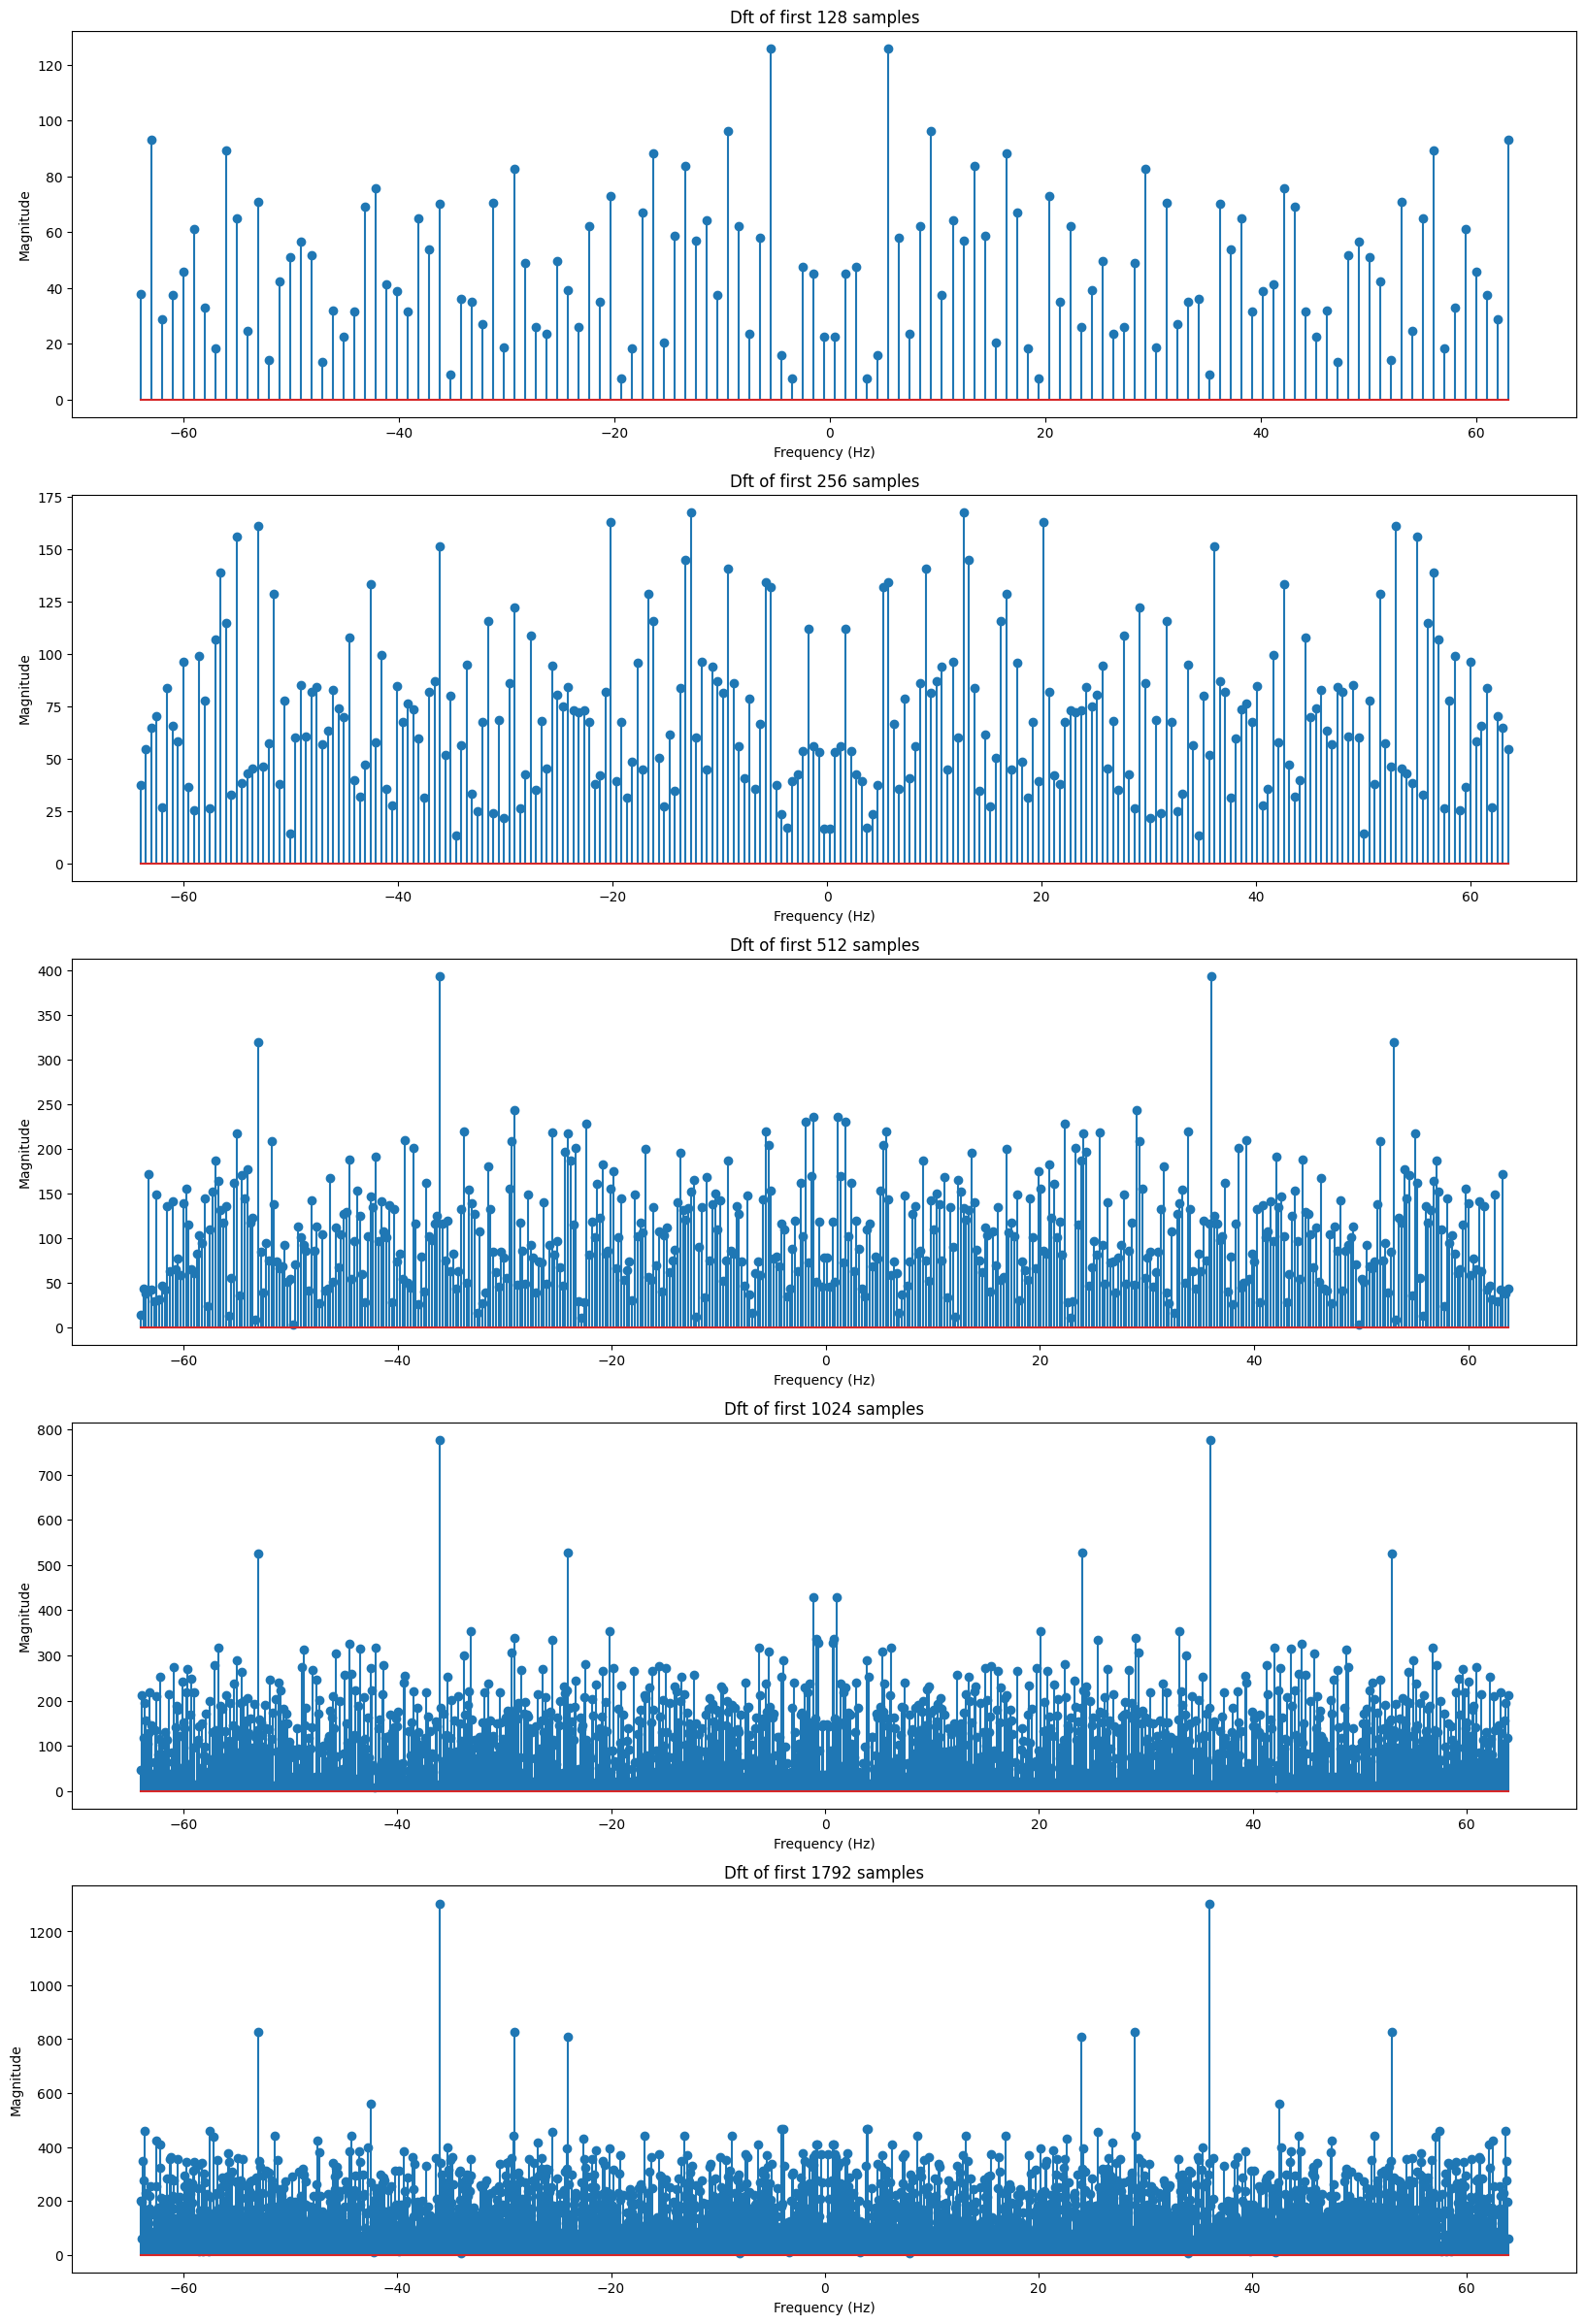
\includegraphics[width=1.0\linewidth]{images/2.png}
    \caption{DFT for first 128,256,512,1024,1792 samples}
\end{figure}}

\newpage

Above showed images are the results for the first part of the question,
where we asked to extract the first 128,256,512,1024,1792 samples from the given signal and find the DFT of those samples.
As we can clearly see from the above images, \textbf{the DFT of the first 128 samples is not enough} to find the harmonic frequencies of the signal. The reason for this , \textbf{we are sampling at different points which may not capture the harmonic frequencies.} And the sampling points increases with the lenght of the signal. Therefore by this \textbf{may capture any missed frequency components.}
And with the \textbf{increase of the signal length} we can see that the \textbf{DFT is getting more and more comprehensible} where we can see the harmonics distinctively.\\
\\
And for the second part of the question we were asked to find the harmonic frequencies of the signal using DFT averaging technique.
Following to this these are the procedures of \textbf{DFT Averaging}

\begin{itemize}
    \item  Partition the input signal \{x[n], n = 0, 1, 2, ..., N - 1\} into L equal subsets, with each subset
    having K samples. (N = LK)
    \item  Apply DFT to each subset of the samples.
    \item  Calculate the arithmetic mean of the gained sets of DFT sequences.
    \item  Plot the average DFT sequence.
    \item Find the indices with higher frequencies.
\end{itemize}


{\begin{figure}[h]
    \centering
    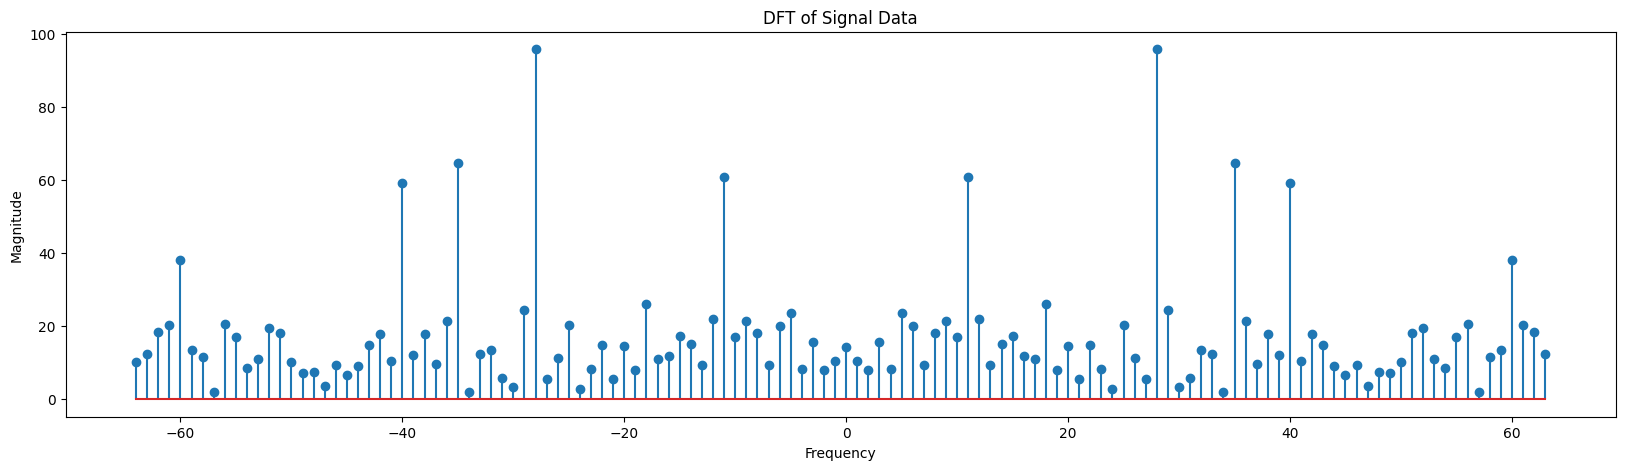
\includegraphics[width=1.0\linewidth]{images/3.png}
    \caption{DFT after averaging, L = 14}
\end{figure}}

{\begin{figure}[h]
    \centering
    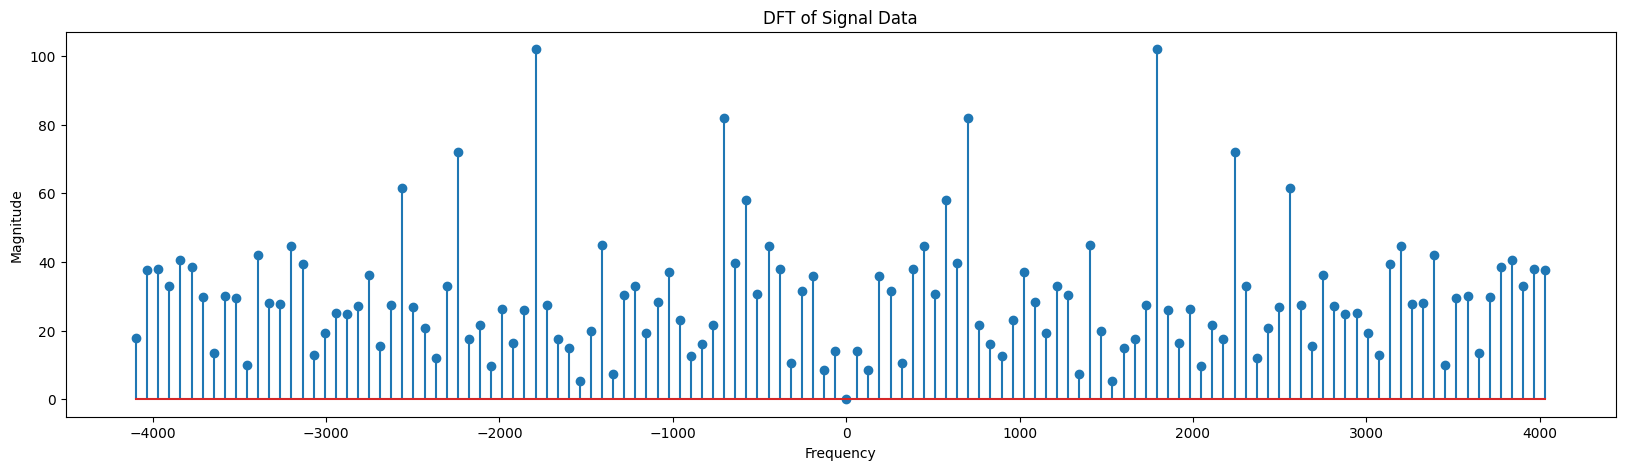
\includegraphics[width=1.0\linewidth]{images/3-3.png}
    \caption{DFT after averaging, L = 4}
\end{figure}}

For the selection of the `L' value with keeping the `K' value as 128. I have tried with different values and found that the \textbf{If we decrease the value less than 4 signal get uncomprehensible to find harmonics.} 

\newpage

{\begin{figure}[h]
    \centering
    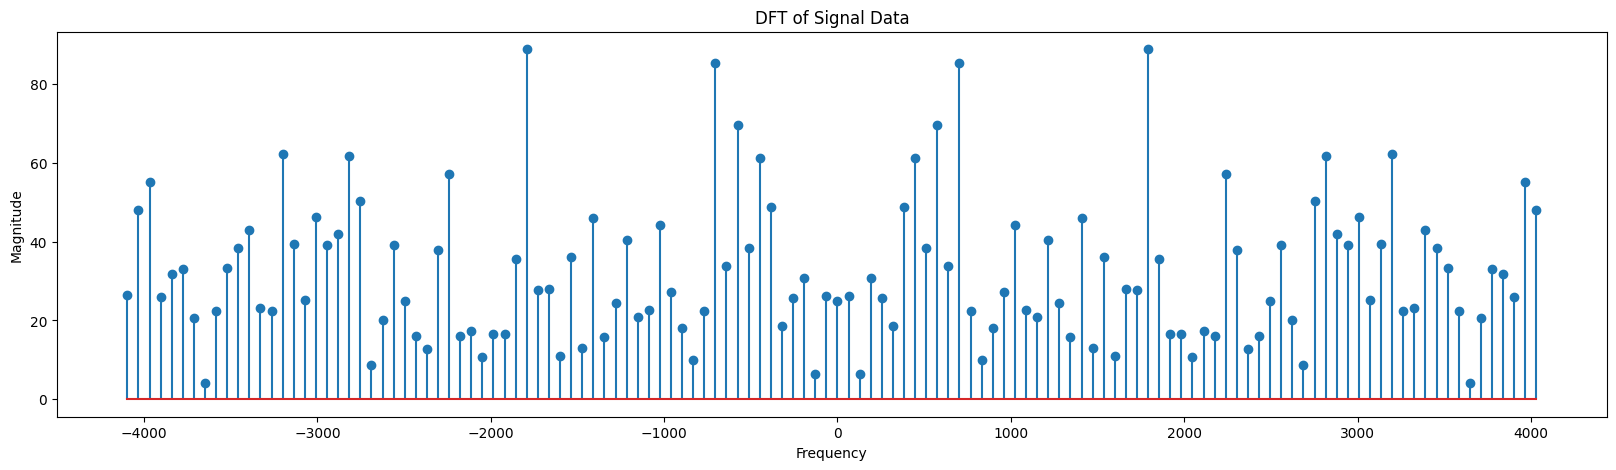
\includegraphics[width=1.0\linewidth]{images/3-5.png}
    \caption{DFT after averaging, L = 3}
\end{figure}}

Following were the harmonic frequencies that I have found from the DFT averaging technique.

\begin{itemize}
    \item Selected harmony 1 : 11 Hz
    \item Selected harmony 2 : 28 Hz
    \item Selected harmony 3 : 35 Hz
    \item Selected harmony 4 : 40 Hz
\end{itemize}


But if we change the value of \textbf{`K' to 100} we cannot see the harmonics more clearly.
And on the other hand if we increase the values of `L' we can see that the \textbf{harmonics are getting more and more worse} with along the \textbf{computational complexity is getting higher and higher}.\\

{\begin{figure}[h]
    \centering
    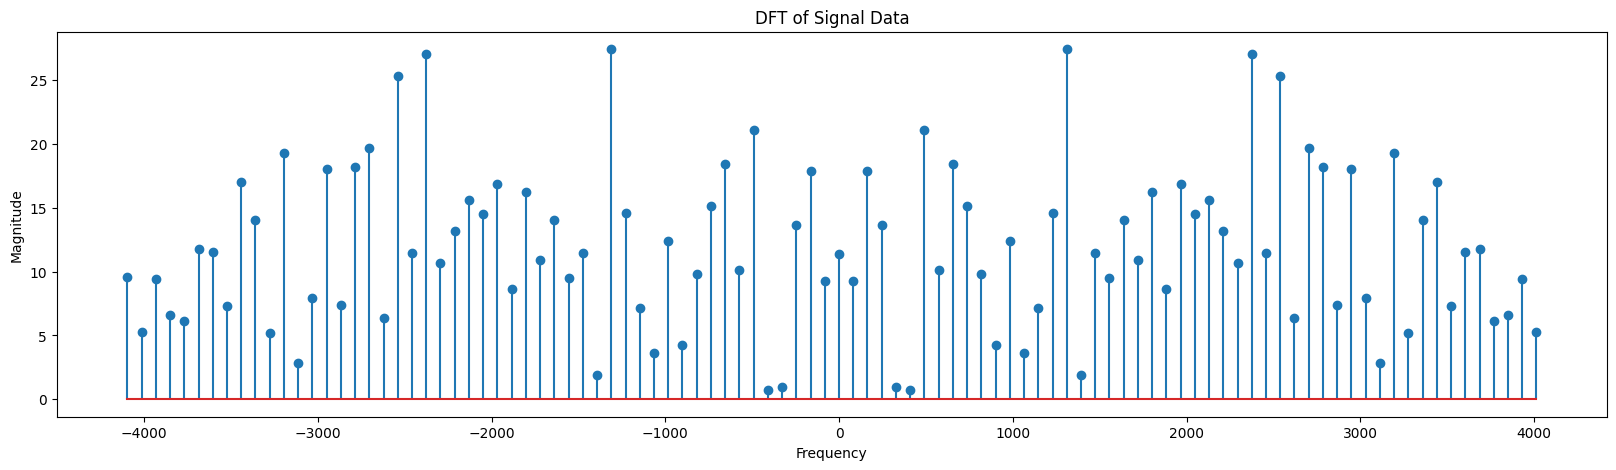
\includegraphics[width=1.0\linewidth]{images/3-2.png}
    \caption{DFT after averaging, K =100}
\end{figure}}

% For the values of `K' we need to select values such that the \textbf{whole signal is captured by the all subsets with same number of samples}. For an example if we take the subset sample size as 100 there will be 92 samples left in the end. which may lead for an erraneous computation.
K represents the subset length, remaining constant across all subsets. It dictates how many samples are in each subset. When the sampling frequency is 128 Hz and K is set to 128, \textbf{each subset encompasses a full signal cycle, with all samples being identical in content.}
However, using different K values like 100 or 135 leads to issues. With K is not equal to 128, subsets may not capture complete signal cycles, causing sample misalignment. This misalignment disrupts harmonic contributions across subsets. For example, when K = 100, the first sample in one subset may not align with the same point in the signal cycle as the first sample in another subset, making harmonic extraction challenging during averaging in methods like DFT.

\newpage

\section{Signal Interpolation Using DFT}

In this task we were given with a audio signal. We were asked to get the first 20000 samples 
from that audio signal and create further more small sub sample arrays. These arrays are similar
to the original array where there are some data loss in the produced sub-arrays.
\\
\\
Our task was simple. We need to re-construct the original signal from the corrupted or else data-missed signal.
for that we need to take the discrete fourier transform of the subsets, Interpolate it with zeroes and find the inverse
DFT and compare with our original singal.


{\begin{figure}[h]
    \centering
    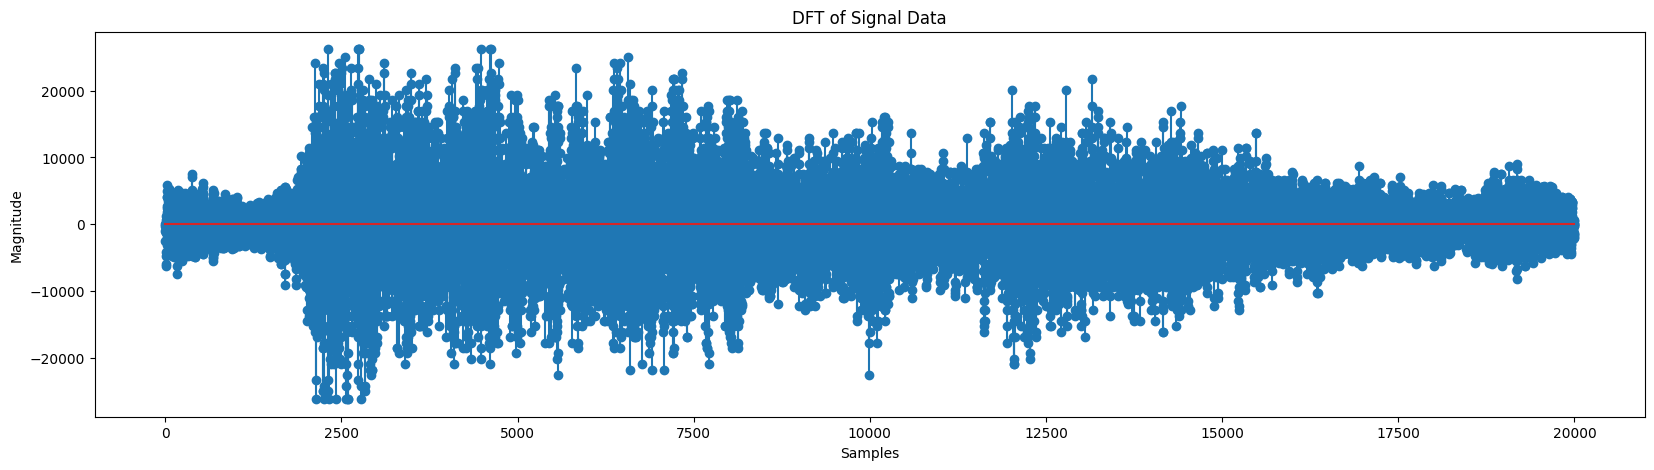
\includegraphics[width=1.0\linewidth]{images/4.png}
    \caption{Extracted Samples from Audio}
\end{figure}}

{\begin{figure}[h]
    \centering
    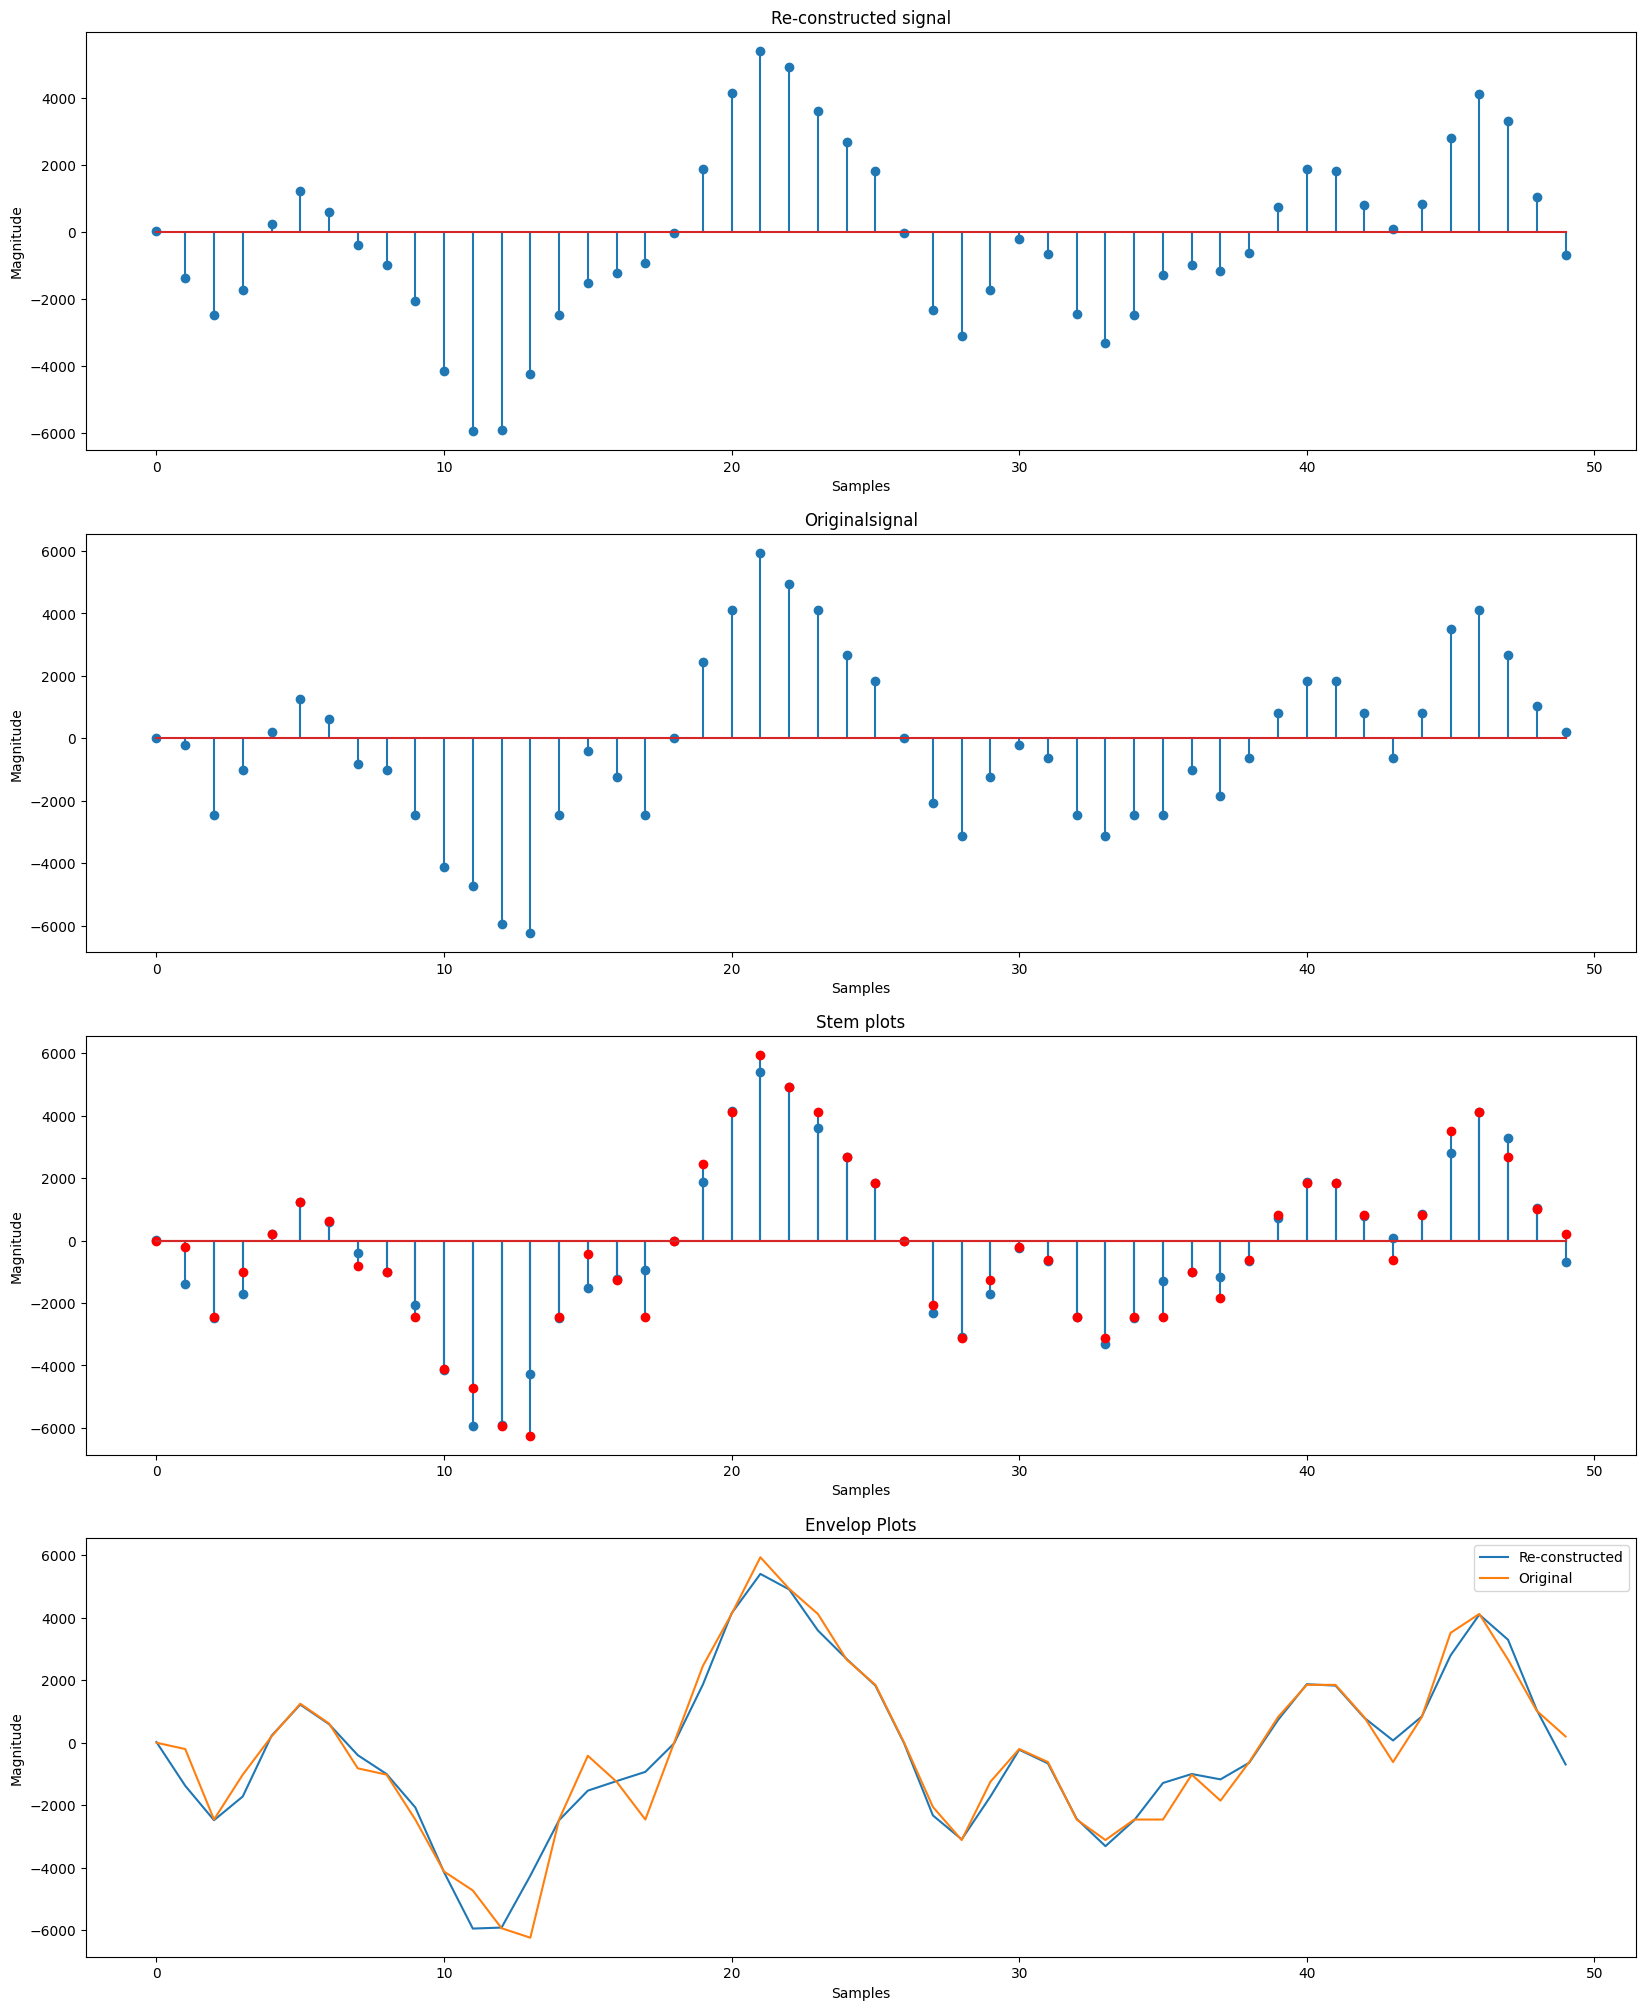
\includegraphics[width=1.0\linewidth]{images/5-1.png}
    \caption{Reconstructed Signal by Interpolating x\_2[n] where k = 1}
\end{figure}}

\newpage

{\begin{figure}[h]
    \centering
    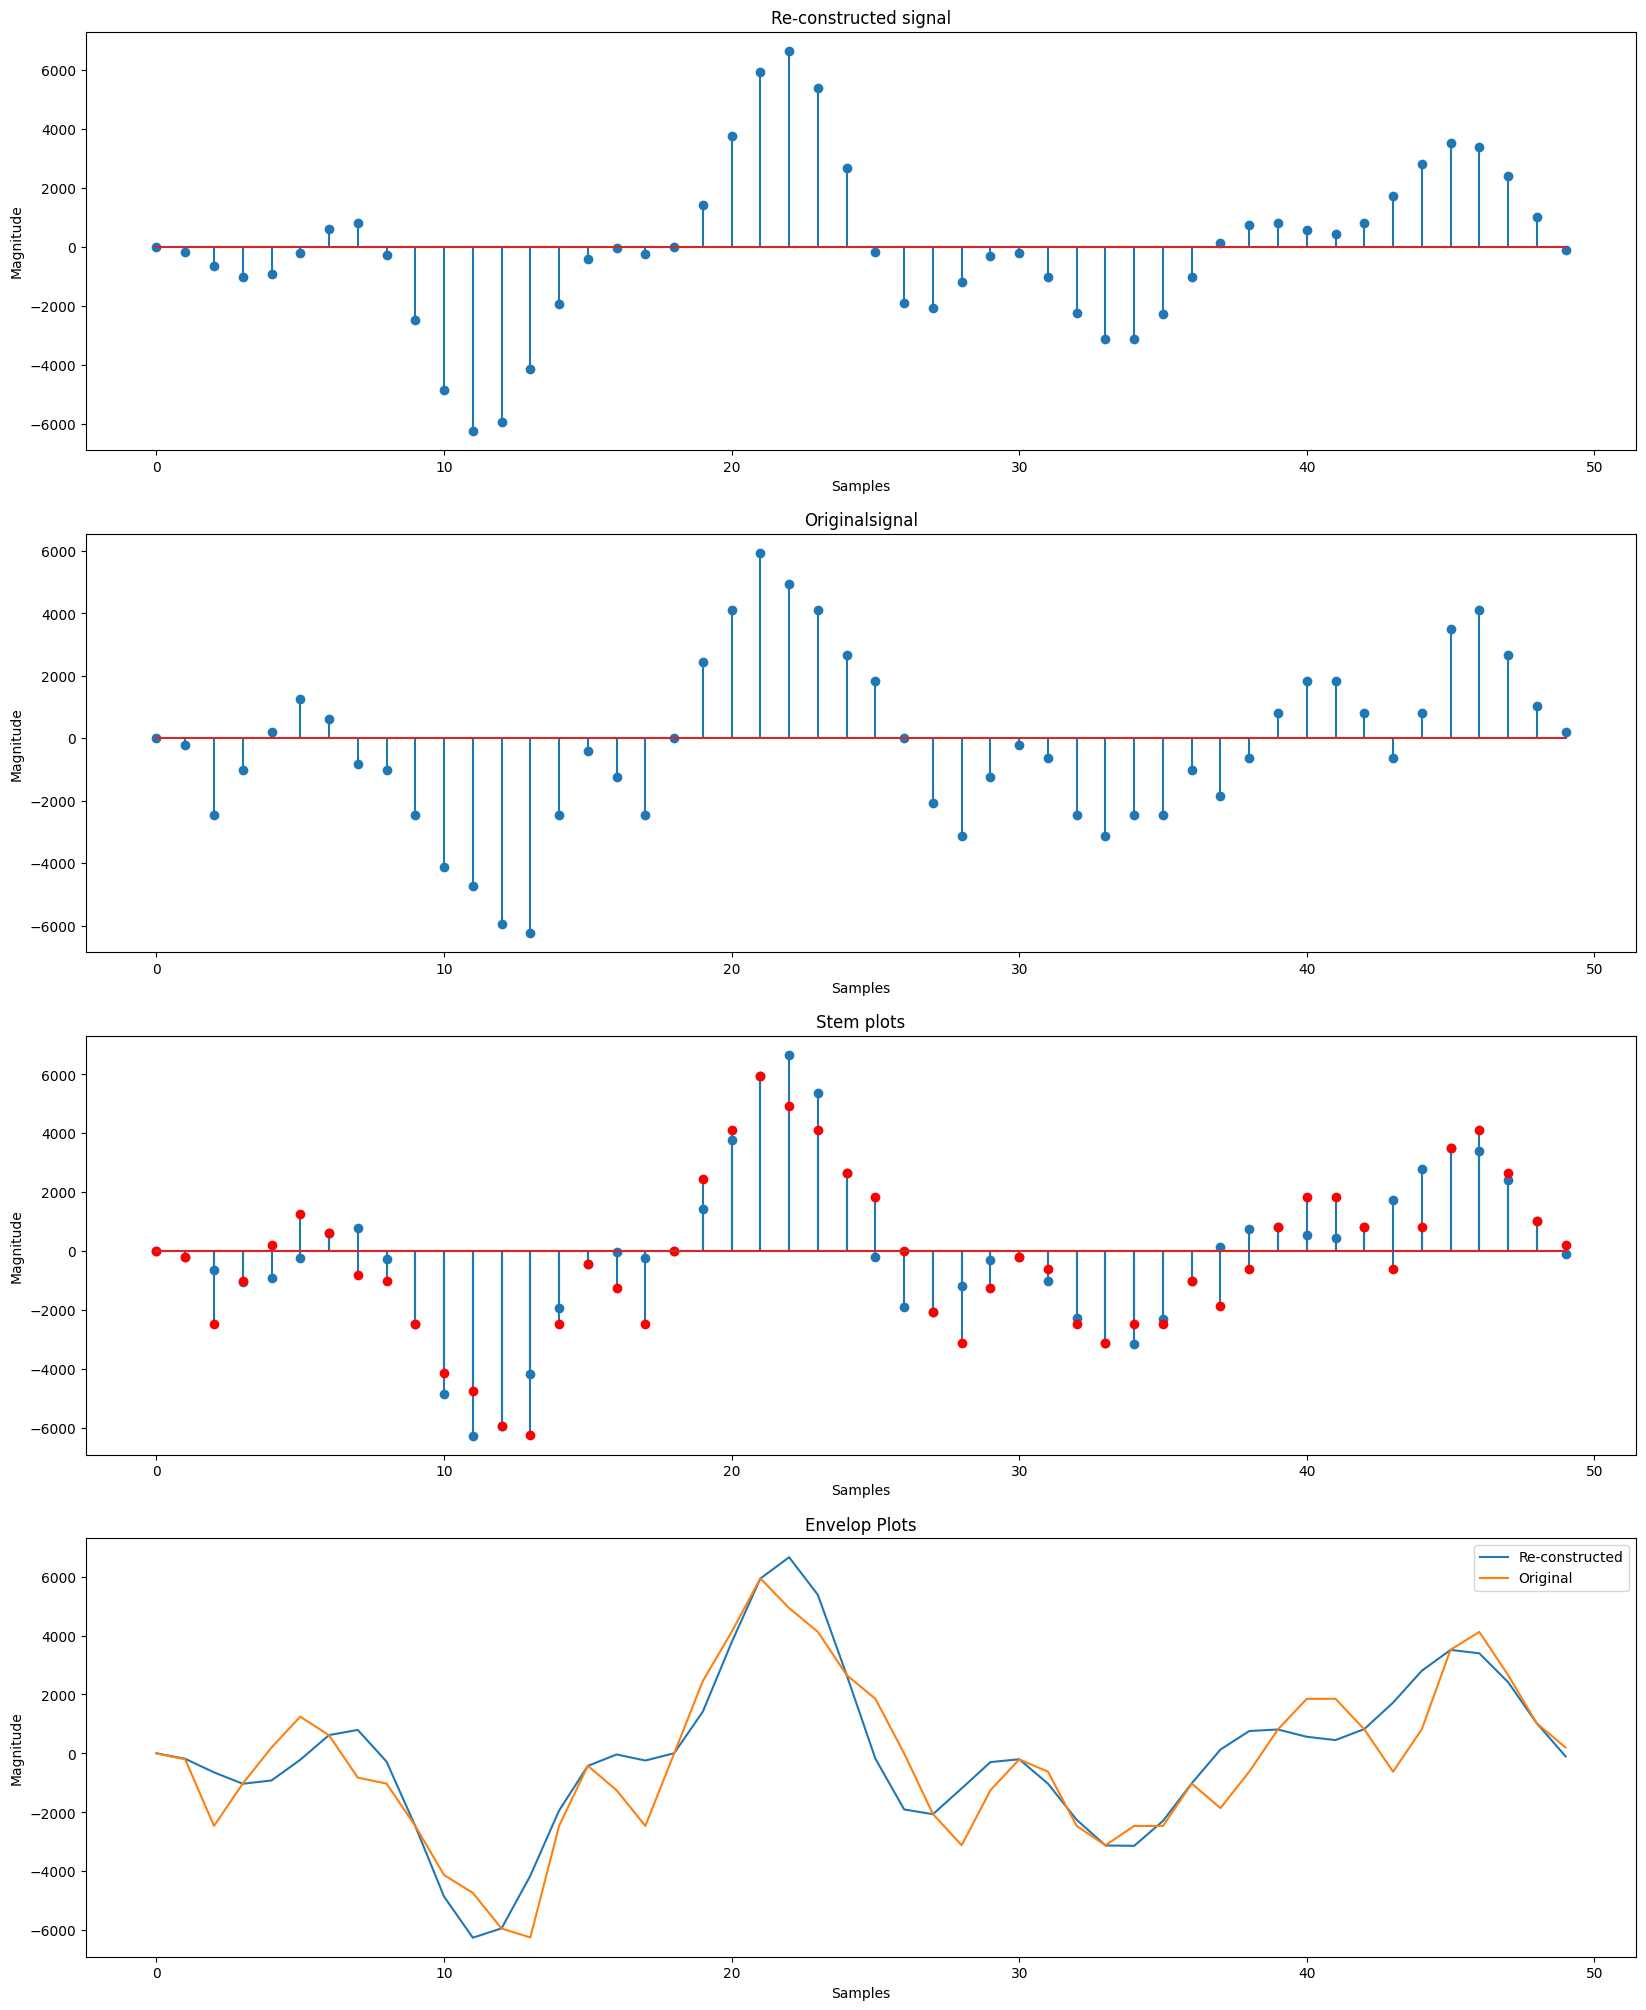
\includegraphics[width=1.0\linewidth]{images/5-2.png}
    \caption{Reconstructed Signal by Interpolating x\_3[n] where k = 2}
\end{figure}}

2-Norm values of the differences
\begin{itemize}
    \item between x and x\_2 : 4.065
    \item between x and x\_3 : 7.883
    \item between x and x\_4 : 9.267
\end{itemize}

From the above results we can see that we have a \textbf{lower norm value for the x\_2 signal.}
Therefore we can say that the difference between the values of the original signal and x\_2 signal is less compared to other signals which we gained from the interpolation.
\textbf{Which also shows that x\_2 is the best match for the original signal.}
\newline
\newline
\textbf{Numerical Precision and Data Truncation} may be the cause for the mismatches between the original and re-constructed signal using interpolation method in frequency doamin.

\newpage

{\begin{figure}[h]
    \centering
    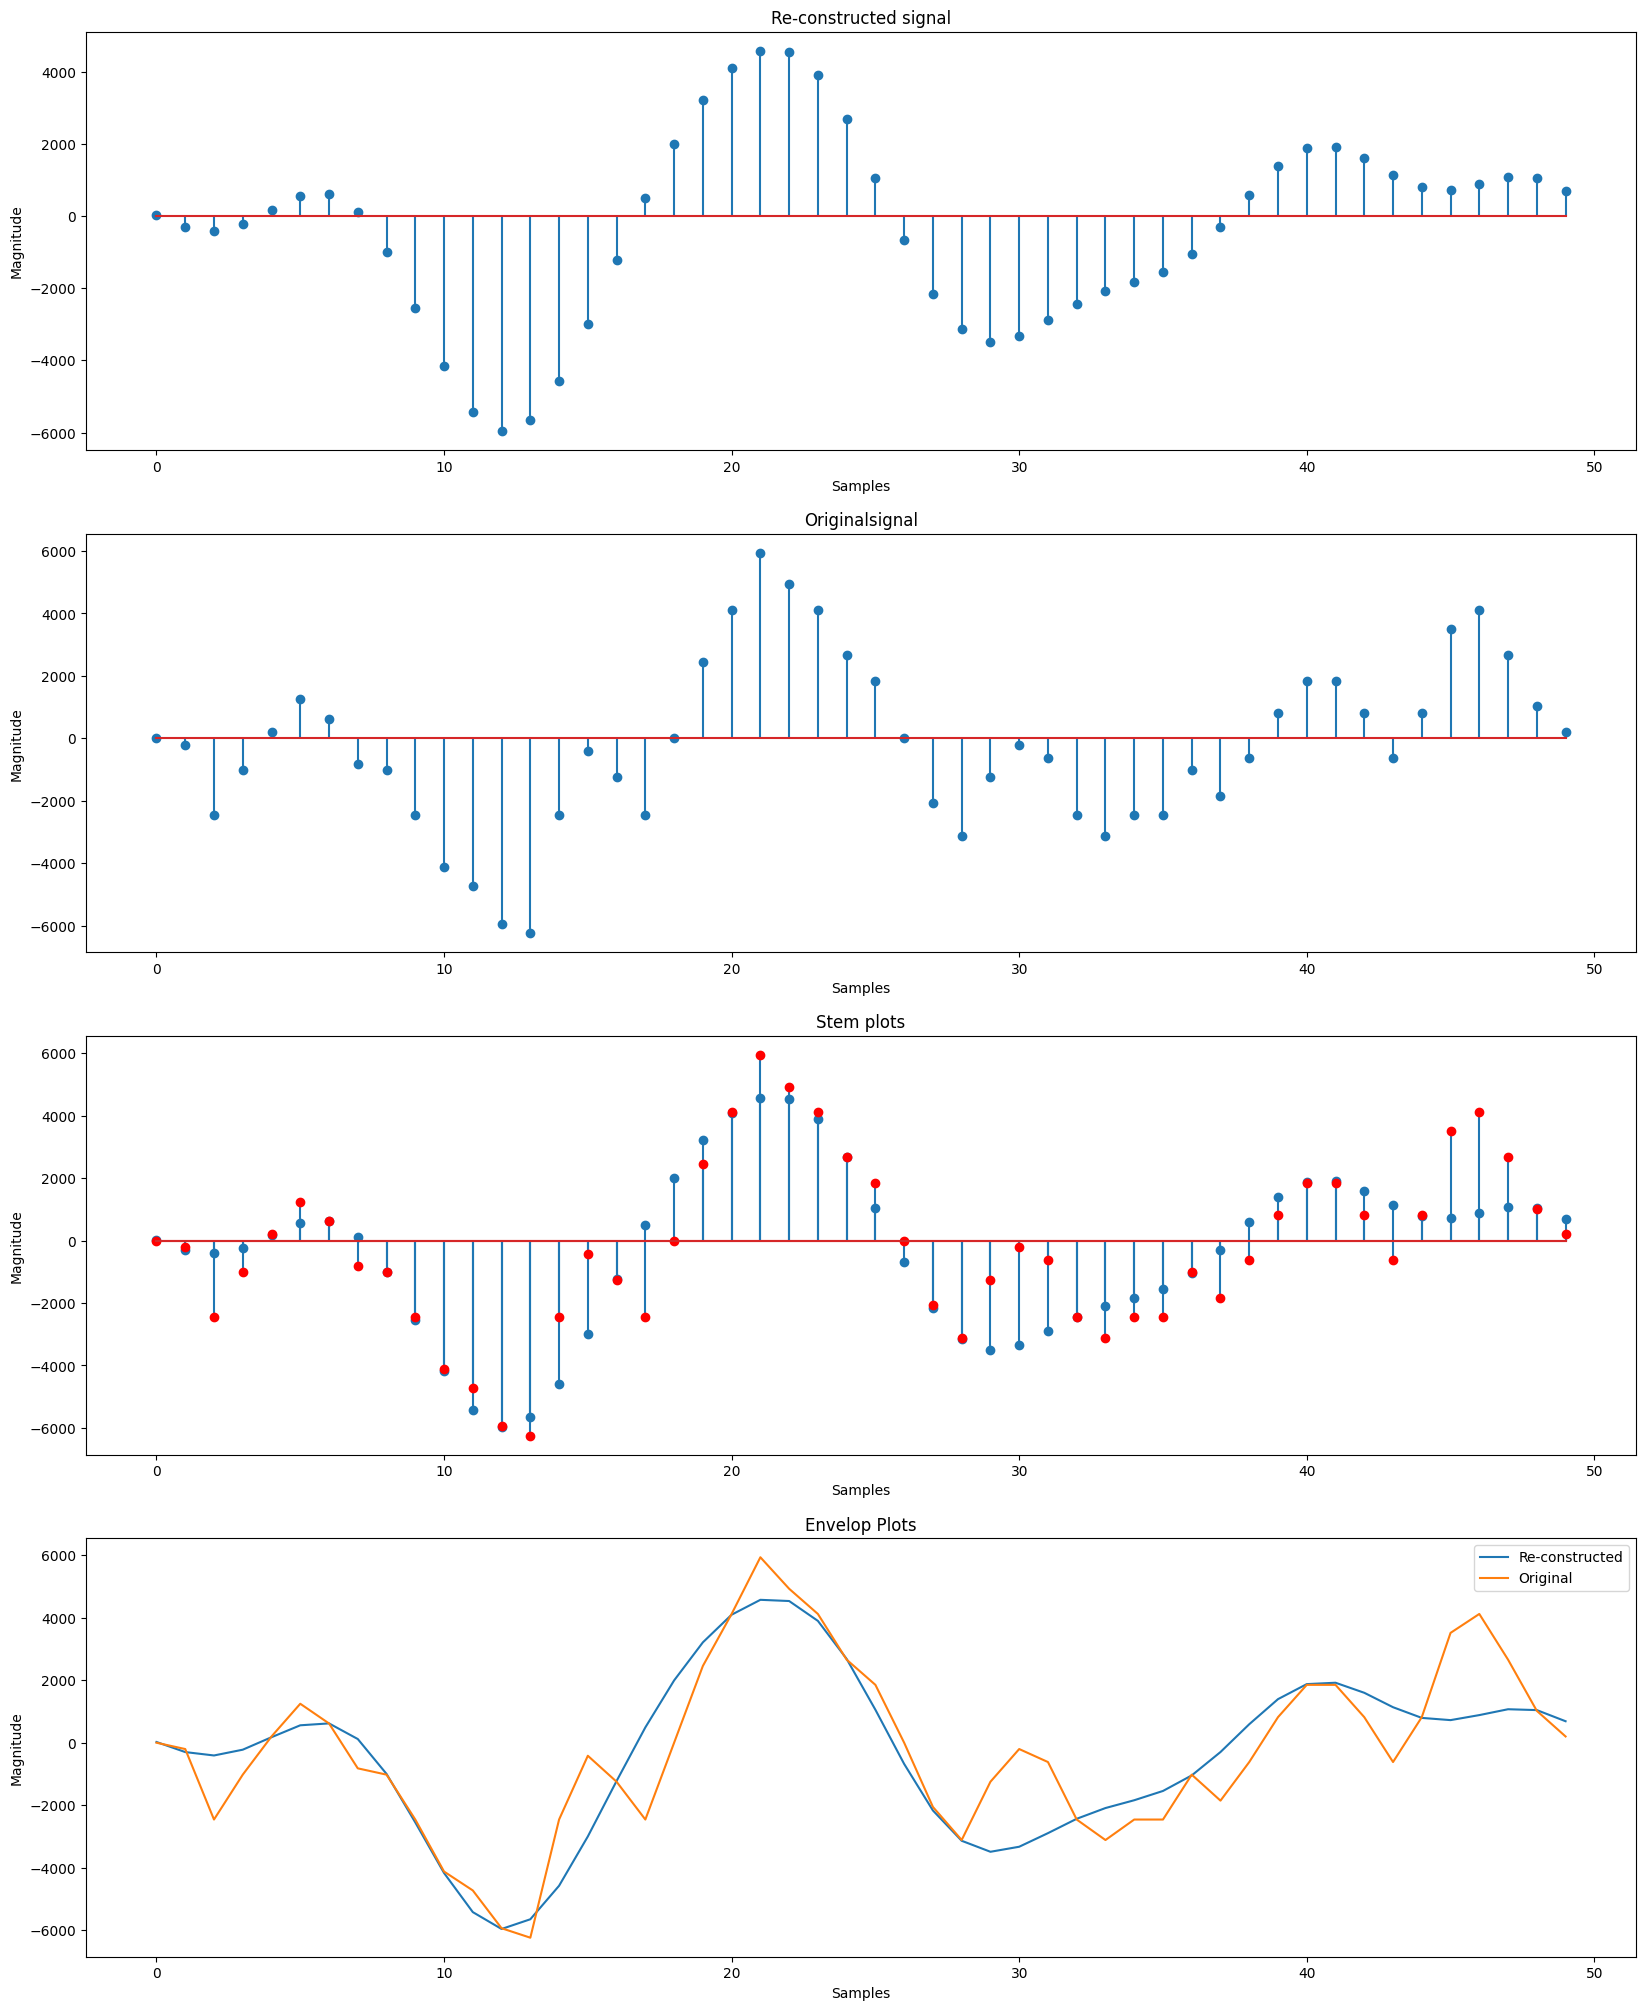
\includegraphics[width=1.0\linewidth]{images/5-3.png}
    \caption{Reconstructed Signal by Interpolating x\_4[n] where k = 3}
\end{figure}}


\section{References}

\begin{itemize}
    \item \href{https://numpy.org/doc/}{Numpy Documentation}
    \item \href{https://www.pearson.com/en-us/subject-catalog/p/discrete-time-signal-processing/P200000003226}{Preferred Text Book}
    % \item \href{ }{Github/EN3160_Assignment_01}
   
\end{itemize}

\section{Github Repository}

Following is the link to my Github repository for this assignment.\\

\href{https://github.com/Vgr20/EN_3551_Assignment_01.git}{Github/EN3551\_Assignment\_01}


\newpage

\twocolumn
\section{Appendix}

\textbf{Code for Task 01}

\lstset{style=mystyle}
\lstinputlisting[language=Octave]{code1.py}

\newpage

\textbf{Code for the Task 02}

\lstset{style=mystyle}
\lstinputlisting[language=Octave]{code2.py}

\end{document}




%%%%%%%%%%%%%%%%%%%%%%%%%%%%%%%%%%%%%%%%%%%%%%%%%%%%%%%%%%%%%%%%%%%%%%%%%%%%%%%%%%%%%%%%%%%%%%%%%%%%%%%%%%%%%%%%%%%%%%%%%%%%%%%%%%%%%%%%%%%%%%%%%%%%%%%%%%%%%%%%%%%%%%%%%%

% {\begin{center}
% \begin{tabular}{ | m{1.85cm} | m{0.85cm}| m{0.85cm} | m{0.85cm} | m{0.85cm} | m{0.85cm} | } 
%  \hline
%  Objectives& Weight & Design 01 & Design 02 & Design 03 & Design 04 \\  
%  \hline\hline
%  Efficiency & 10 & 7 & 8 & 8 & 9 \\
%  \hline
%  Mobility & 10 & 7 & 9 & 8 & 8 \\
%  \hline
%  Easy Maintenance & 10 & 7 & 6 & 5 & 8 \\
%  \hline
%  Refilling accessibility & 5 & 3 & 3 & 2 & 4 \\
%  \hline
%  Durability & 5 & 2 & 3 & 3 & 2 \\
%  \hline
%  Manufacture cost & 5 & 3 & 3 & 2 & 3 \\
%  \hline
%  Overall Look & 5 & 2 & 3 & 5 & 2 \\
%  \hline
%  \hline
%  Total & 50 & 31 & 35 & 33 & 36 \\
%  \hline
 
% \end{tabular}
% \end{center}}

%%%%%%%%%%%%%%%%%%%%%%%%%%%%%%%%%%%%%%%%%%%%%%%%%%%%%%%%%%%%%%%%%%%%%%%%%%%%%%%%%%%%%%%%%%%%%%%%%%%%%%%%%%%%%%%%%%%%%%%%%%%%%%%%%%%%%%%%%%%%%%%%%%%%%%%%%%%%%%%%%%%%%%%%%%


% \begin{center}
% \begin{tabular}{ | m{2cm} | m{5cm}| m{2cm} | m{6cm} | } 

%  \hline
%  Part Name & Description & Supplier & Part Link\\  
%  \hline\hline
%  NE555P & 8-pin Precise timer & Texas Instruments & \href{https://www.lcsc.com/product-detail/Timers-Clock-Oscillators_Texas-Instruments-NE555P_C46749.html}{NE555p data sheet}\\
%  \hline
%  2N2222A & Generic npn transistor & Slkor & \href{https://www.lcsc.com/product-detail/Bipolar-Transistors-BJT_Slkor-SLKORMICRO-Elec-2N2222A_C5330385.html}{2N2222A data sheet}\\
%  \hline
%   LM7805 & Linear voltage Regulators & LRC & \href{https://www.lcsc.com/product-detail/Linear-Voltage-Regulators-LDO_LRC-LR7805_C2846986.html}{Lm7805 Data sheet}\\
%  \hline
%   HC sr501 & Passive IR sensor & HC & \href{https://www.lcsc.com/product-detail/Timers-Clock-Oscillators_Texas-Instruments-NE555P_C46749.html}{HC sr501 data sheet}\\
%  \hline
%   KNSCHA ZE11000UF & 1000uF Capacitor & KNSCHA & \href{https://www.lcsc.com/product-detail/Solid-Capacitors_KNSCHA-ZE11000UF35V119EC0014_C2992586.html}{Capacitor data sheet}\\
%  \hline
%   Resistors & Resistors with different values & Texas Instruments & \href{https://www.lcsc.com/search?q=resistors%20through%20hole}{Through hole resistors}\\
%  \hline
 
% \end{tabular}  
% \end{center}
%%%%%%%%%%%%%%%%%%%%%%%%%%%%%%%%%%%%%%%%%%%%%%%%%%%%%%%%%%%%%%%%%%%%%%%%%%%%%%%%%%%%%%%%%%%%%%%%%%%%%%%%%%%%%%%%%%%%%%%%%%%%%%%%%%%%%%%%%%%%%%%%%%%%%%%%%%%%%%%%%%%%%%%%%%